\chapter{Background Physics}

\graphicspath{{images/background/}}

\section{Introduction to solar physics}

\subsection{Layers of the Sun}

The radius of a star is estimated as the radius at which the optical depth, a measure of the opacity of a plasma, takes the value $2/3$. In our own Sun, this layer is found at a radius of approximately $R_{\odot} = 695,508$km and is known as the photosphere. Below this layer lie the three inner regions: the core, the radiative region and the convection zone. From the centre to around $0.2 R_{\odot}$ lies the engine of the Sun, the core, undergoing fusion and producing the energy fuelling the [TODO rest of the Sun]. Between the core and the convection zone (at $0.71R_{\odot}$) is the radiative zone, the region at which the density gradient is high enough that the plasma is stable to convective instabilities. Heat is transported from the core through the radiative zone mostly through the process of radiative transfer. Between the radiative zone and the photosphere lies the conduction zone, the region at which the density gradient is no longer able to stabilise the plasma against the effect of the negative temperature gradient and convection occurs. The convection within this region drives the solar dynamo and, thus, the creation of the solar magnetic field.

Above the photosphere lies the atmosphere of the Sun, consisting of the photosphere, chromosphere, transition region and corona. The photosphere, usually referred to as the surface of the Sun, has a temperature of approximately $6000$K and radiates most of the visible light emitted from the Sun. As a result the photosphere is the only part of the Sun usually visible by the human eye (the exception being during eclipses when both the chromosphere and corona can be seen). Just above the photosphere is the chromosphere, extending beyond the surface by $3000$--$5000$km. The temperature ranges between $6000$K at the photospheric boundary, a minimum of $3500$K internally, and $25,000$K approaching the transition region. This narrow layer of depth $100$km lies between the chromosphere and the solar corona and is the point at which the nature of the physics in the solar atmosphere changes rapidly with height. The primary difference is in the extreme temperature difference across the layer, typically ranging from $25,000$K on the chromospheric side, to over $1,000,000$K on the coronal side. TODO mention temperature catastrophe? This coincides with a drop in density of the layer, from TODO to TODO. The other major difference is in the dominance of certain types of dynamics. While the dynamics of the chromosphere are dominated by the fluid dynamics of the plasma, and merely influenced by the magnetic field, the dynamics of the solar corona are dominated by magnetic forces.

TODO emphasise focussing on the corona over other layers

\subsection{Coronal heating problem}

refer to Browning, Hood, Klimchuck

\section{MHD Equations}

\subsection{The Navier-Stokes equations}

TODO

\subsection{Magnetohydrodynamics and the induction equation}

Magnetohydrodynamics (MHD) describes electrically conducting fluids, that is fluids which interact with electromagnetic fields. Typical examples of such fluids are plasmas and molten metals, the investigation of the latter being key to the understanding of the Earth's molten outer core and its associated magnetic dynamo. In contrast, the Earth's mantle, being made of electrically insulating magma, does not interact with the Earth's magnetic field and is not typically modelled as a magnetohydrodynamic fluid. Both small-scale laboratory plasmas, such as those found in current fusion devices, and large-scale astrophysical plasmas, such as those in the interstellar medium, can be effectively modelled using the MHD equations. While the MHD equations have a large range of applicability, they are limited to systems with dynamics at length-scales much larger than the ion skin depth or Larmor radius, and time-scales much longer than the ion gyration time. For these systems, a kinetic approach using the Vlasov or Boltzmann equations is more appropriate. The ideal MHD equations can be recovered from the Boltzmann equation by taking appropriate moments, however we choose to take a more traditional, fluid-based approach here.

The magnetohydrodynamic equations are a synthesis of the Navier-Stokes equations of fluid dynamics and Maxwell's equations of electromagnetism. The latter set of equations describes the generation of an electric field $\vec{E}$ by a charge density $\rho_c$ through Gauss's law,
\begin{equation}
  \label{eq:gauss_law}
 \nabla \cdot \vec {E} ={\frac {\rho_c }{\varepsilon _{0}}},
\end{equation}
the non-existence of monopoles in the magnetic field $\vec{B}$,
\begin{equation}
  \label{eq:gauss_law_for_magnetism}
  \nabla \cdot \vec {B} =0,
\end{equation}
the generation of electric fields due to changes in the magnetic field in time $t$ through the Maxwell-Faraday equation,
\begin{equation}
  \label{eq:maxwell_faraday}
 \nabla \times \vec {E} =-{\frac {\partial \vec {B} }{\partial t}},
\end{equation}
and the generation of magnetic fields due to currents $\vec{\jmath}$ and changing electric fields through Ampère's law,
\begin{equation}
  \label{eq:ampere_law}
 \nabla \times \vec {B} =\mu _{0}\left(\vec {\jmath} +\varepsilon _{0}{\frac {\partial \vec {E} }{\partial t}}\right).
\end{equation}
Written in SI units, these equations use the permittivity $\varepsilon_{0}$ and permeability $\mu_0$ of free space.

Many conducting fluids can be considered electrically neutral, that is on the timescale of fluid motion the charges within the fluid are able to quickly redistribute to nullify any electric forces. This is true for coronal plasmas where the electrons, being much lighter than the ions, are able to very quickly redistribute. This allows Gauss's law to be entirely neglected. The displacement current, the last term in Ampère's law, can also be neglected due to the assumption that fluid motions are non-relativistic, that is the typical fluid velocity is much less than the speed of light, $c$. In order to couple the fluid motion to the electromagnetic fields, a constitutive Ohm's law is also included which describes the generation of currents in response to electric fields. This eventually allows the complete elimination of $\vec{E}$ from the governing equations. In a fluid's rest frame, the current response to an electric field $\vec{E}'$ is
\begin{equation}
  \label{eq:rest_frame_ohms_law}
  \vec{\jmath} = \sigma \vec{E}',
\end{equation}
where $\sigma$ is the (finite) conductivity of the fluid. The Lorentz transformation to the frame where the fluid is moving at velocity $\vec{u}$ is
\begin{equation}
  \label{eq:resistive_ohms_law}
  {\vec {E}}+{\vec{u}}\times {\vec {B}}=\eta{\vec {\jmath}},
\end{equation}
where we have rewritten the conductivity as the resistivity $\eta = 1/\sigma$. In the limit of perfect, or infinite, conductivity, Ohm's law is written,
\begin{equation}
  \label{eq:ideal_ohms_law}
  {\vec {E}}+{\vec{u}}\times {\vec {B}}=0.
\end{equation}

Combining the remaining parts of Ampère's law, the Maxwell-Faraday equation, and the resistive Ohm's law results in the induction equation,
\begin{equation}
  \label{eq:nonsimple_induction_equation}
{\frac {\partial \vec {B} }{\partial t}} = \nabla \times (\vec{u} \times \vec{B}) - \nabla \times (\eta/\mu_0 \nabla \times \vec{B}),
\end{equation}
which, in the limit of uniform resistivity, may be written
\begin{equation}
  \label{eq:induction_equation}
{\frac {\partial \vec {B} }{\partial t}} = \nabla \times (\vec{u} \times \vec{B}) - \frac{\eta}{\mu_0}\nabla^2 \vec{B}.
\end{equation}
This equation essentially describes the advection and generation of a magnetic field due to fluid motions and the diffusion of the field due to resistivity. The magnetic field must still satisfy the solenoidal constraint $\nabla \cdot \vec{B}$.

Additional non-ideal physics like ambipolar diffusion and the Hall effect can be modelled through additional terms in Ohm's law, however in the solar corona these effects are small compared to resistivity so they are neglected.

\subsection{The non-dimensionalised MHD equations}

Combining the fluid equations[TODO ref] and the induction equation, we now write the full set of MHD equations in their non-dimensionalised form
\begin{gather}
%\begin{equation}
\label{eq:mhda}
\frac{D\rho}{Dt} = - \rho \vec{\nabla} \cdot \vec{u},\\
%\end{equation}
%\begin{equation}
\rho\frac{D\vec{u}}{Dt} = -\vec{\nabla} p + \vec{\jmath} \times \vec{B} + \vec{\nabla} \cdot \ten{\sigma},\\
%\end{equation}
%\begin{equation}
\frac{D\vec{B}}{Dt} = (\vec{B} \cdot \vec{\nabla})\vec{u} - (\vec{\nabla} \cdot \vec{u})\vec{B} + \eta \nabla^2 \vec{B},\\
%\end{equation}
%\begin{equation}
\rho\frac{D\varepsilon}{Dt} = -p \vec{\nabla} \cdot \vec{u} + {Q}_{\nu} + {Q}_{\eta},%\\
\label{eq:energy}
%\end{equation}
\end{gather}
where $\vec{u}$ is the plasma velocity, $\vec{\jmath} = \nabla
\times \vec{B}$ is the current density, $\ten{\sigma}$ is the viscous
stress tensor, $\eta = 1/S$ is the normalised resistivity (equivalent
to the inverse of the Lundquist number $S$), and use has been made of
the material derivative, $D/Dt = \partial/\partial t + (\vec{u} \cdot
\vec{\nabla})$. The internal energy density is given by the equation of state for an ideal gas
\begin{equation}
\varepsilon = \frac{p}{\rho(\gamma - 1)},
\end{equation}
where the specific heat ratio is given by $\gamma = 5/3$. The
  terms ${Q}_{\nu} = \ten{\sigma} : \vec{\nabla}\vec{u}$ and
  ${Q}_{\eta} = \eta | \vec{\jmath} |^2$ model Ohmic heating and viscous heating, respectively.

Using the nondimensionalisation scheme found
in~\cite{arberStaggeredGridLagrangian2001}, reference values for the
magnetic field $B_0$, length $L_0$ and density $\rho_0$ are chosen to
align with values typical for a coronal loop. The problem domain is
non-dimensionalised to $[-2,2] \times [-2,2] \times [-10,10]$ in the
$x$, $y$ and $z$-directions, respectively. Velocity and time are
non-dimensionalised using the Alfv\'en speed $u_A = B_0 / \sqrt{\rho_0
  \mu_0}$ and Alfv\'en crossing time $t_A = L_0/u_A$,
respectively. Temperature is non-dimensionalised via $T_0 = u_A^2
\bar{m} / k_B$, where $k_B$ is the Boltzmann constant and $\bar{m}$ is
the average mass of ions, here taken to be $\bar{m} = 1.2m_p$ (a mass
typical for the solar corona) where $m_p$ is the proton mass. The
reference values of other variables are derived from these
quantities and are listed in Table~\ref{tab:reference-values}. Dimensional quantities can be recovered by multiplying the non-dimensional variables by their respective reference value (e.g. $\vec{B}_{\dim} = B_0 \vec{B}$). All further reference to variables will be to their non-dimensionalised values, unless stated otherwise.

\section{Anisotropic Viscosity}

\subsection{Viscosity}

Physically, viscosity is the internal friction of a fluid arising due to interactions (typically collisions) between the particles making up the fluid. Within the context of MHD, viscosity provides two functions. The first is momentum transport, included in the momentum equation as the divergence of the viscous stress tensor $\ten{\sigma}$, written using Einstein notation for clarity,
\begin{equation}
  \label{eq:viscous_momenum_transport}
  (\nabla \cdot \ten{\sigma})_j = \frac{\partial}{\partial x_i} \sigma_{ij}.
\end{equation}

In three dimensions, the nine components of $\sigma$ quantify the flux (due to viscosity) of each component of momentum in each direction of motion. For example, the $\sigma_{xy}$ component gives the flow of $x$-momentum in the $y$-direction. Due to symmetry arising from viscosity naturally conserving angular momentum, the tensor is itself symmetric, so the component $\sigma_{xy}$ also quantifies the flow of $y$-momentum in the $x$-direction.

The second function of viscosity is to convert kinetic into thermal energy through work done by local deformations. This is encoded in a term in the energy equation of the MHD equations, again expressed in Einstein notation,
\begin{equation}
  \label{eq:viscous_heat_generation}
  \ten{\sigma} : \nabla \vec{u} = \sigma_{ij} \frac{\partial u_i}{\partial x_j}.
\end{equation}

Beyond the physical requirement of conservation of angular momentum, it is assumed that Stokes' hypothesis holds, that is bulk viscosity is zero and viscosity does not act under uniform compression or expansion of the fluid. This requires the viscous stress tensor to be trace-free,
\begin{equation}
  \label{eq:trace_free_tensor}
  \text{tr}(\ten{\sigma}) = 0.
\end{equation}

Many fluids encountered in nature are Newtonian fluids, that is the viscous stress arising from any deformation of the fluid is directly proportional to the rate of strain of the deformation,
\begin{equation}
  \label{eq:isotropic_viscous_tensor}
  \ten{\sigma} = \nu \ten{W},
\end{equation}
where the traceless strain rate tensor $\ten{W}$ is written as
\begin{equation}
  \label{eq:rate_of_strain}
  \ten{W} = \nabla\vec{u} + (\nabla\vec{u})^T - \tfrac{2}{3}(\nabla \cdot \vec{u})\ten{I}.
\end{equation}
As a result of a viscous stress tensor being symmetric and traceless, we may alternatively write the viscous heating term, equation~\ref{eq:viscous_heat_generation} as
\begin{equation}
  \label{eq:viscous_heat_generation2}
  \ten{\sigma} : \nabla \vec{u} = \frac{1}{2} \ten{\sigma} : \ten{W}.
\end{equation}

\subsection{Anisotropic viscous tensors}

The form of the viscous stress tensor in a magnetized plasma has been derived in a number of ways, to varying degrees of accuracy. The derivations typically use the methods of kinetic theory, taking moments of the Boltzmann-Maxwell equations, to arrive at approximations to the viscosity, among other types of molecular transport. A first approximation of the stress tensor can be found in the 1939 work of Chapman and Cowling~\cite{chapmanMathematicalTheoryNonuniform1970}. Their results show that the stress response to a rate of strain can be split into the responses to three types of motion: compression or dilation along the field, deformations in the plane transverse to the field, and deformations in the plane including the field. The latter two responses can each be further split into two parts, giving five distinct contributions to the stress tensor in total. This natural splitting of the tensor in response to various kinds of strain is discussed in depth by Kaufman~\cite{kaufmanPlasmaViscosityMagnetic1960}. In the same article, Kaufman presents both an illustrative description of the drift and perpendicular components of the tensor, and a derivation of the full tensor from a more simplified Boltzmann equation than is used by Chapman and Cowling. The tensor derived by Braginskii~\cite{braginskiiTransportProcessesPlasma1965} is perhaps the most well known and includes accurate approximations to the five viscous transport parameters. The parallel component of the stress tensor has been derived without use of kinetic theory by Hollweg~\cite{hollwegViscosityMagnetizedPlasma1985}, showing the viscous response to parallel motions to be a result of collisions repartitioning anisotropies in the thermal pressure.

We initially present an overview of Braginskii's simplified derivation of the form and magnitude of the various tensor components. This is given as an intuition-building illustration of the physics rather than a rigorous, mathematical derivation of the tensor, which can be found in~\cite{braginskiiTransportProcessesPlasma1965}. We then present the full Braginskii tensor in the its usual form, a modified form useful for simulations, and the full switching tensor for completeness, relegating the main discussion of the switching tensor to chapter~\ref{chp:switching_model}.

\subsection{Simplified derivation of Braginskii tensor}

In a Newtonian fluid, the motion of a single particle travelling with a typical thermal velocity $v$ and colliding with other particles once in a typical collision time $\tau$ will appear as a number of broken, straight lines, each of approximate length $l = v\tau$, also known as the mean free path. These motions have no preferred direction, resulting in an isotropic transfer of momentum. In contrast, in a plasma made up of charged particles with charge $e$ and mass $m$, threaded by a magnetic field of strength $B$, the particles follow helical paths of approximate radius $r = v/\omega$, where $\omega = eB/m$ is the cyclotron frequency. After a time $\tau$, a typical particle will undergo a collision and its path will describe a new helix. The total resultant motion depends on the strength of the magnetic field. In the presence of a weak field, the radius of the helix may be much larger than the mean free path or, in terms of the cyclotron frequency, $\omega \tau \ll 1$. As a result, the path between collisions will be close to straight and the total path will resemble that of the motion without a magnetic field. In the presence of a strong field, $\omega \tau \gg 1$ and a typical particle will be able to wind around the field a number of times, travelling a distance $l$ along the field, before colliding. As a result the transport of momentum (i.e. viscosity) is strongly anisotropic: unaffected in the direction of the field, but strongly reduced in the transverse direction.

A characteristic coronal value of $\omega \tau$ can be calculated using expressions found in Braginskii~\cite{braginskiiTransportProcessesPlasma1965}. The collision time can be written in SI units as,
\begin{equation}
  \label{eq:collision_time}
  \tau = 0.82 \times 10^{-6} \frac{T^{3/2}}{n},
\end{equation}
and the cyclotron frequency as,
\begin{equation}
  \label{eq:cyclotron_frequency}
  \omega = 0.96\times10^8 B,
\end{equation}
where the Coloumb logarithm has been taken to be 22, and the mass fraction, the ratio of ion to proton mass, $m_f = m_i/m_p$ has been taken to be a typical solar value of $1.2$. The expression for $\tau$ differs from that given by Hollweg~\cite{hollwegViscosityMagnetizedPlasma1985} due to the more accurate inclusion of the mass fraction here. A solar active region could have typical temperatures of around $2\times 10^6$K, and number densities of $n = 3 \times 10^3\text{m}^{-3}$, giving $\tau = 0.773$s. The magnetic field can be as strong as $5\times 10^{-3}$T, giving $\omega = 4.79 \times 10^5 \text{s}^{-1}$, resulting in $\omega \tau = 3.70 \times 10^5$. This indicates viscosity in most of the solar corona is highly anisotropic.

As a basic introduction, I will now present a condensed review of Braginskii's qualitative derivation of the form of the anisotropic viscosity stress tensor in a magnetized plasma, and its associated transport parameters~\cite{braginskiiTransportProcessesPlasma1965}. Consider a plasma where, on average, each particle moves a distance $\Delta x$ in the collision time $\tau$ before colliding. TODO diagram in inkscape. After the collision the particle has equal probability of moving to the left and the right. Since we are concerned with the viscous diffusion of momentum, and not advection, we consider the case where the particle flux through some plane $x=x_0$ is zero (that is the number of particles moving through the plane from the left is equal to the number of particles from the right). This implies a uniform number density in the small layer around $x_0$. We do, however, consider a non-uniform velocity, say $u_y$, which changes slowly enough over the distance $\Delta x$ that we may write
\begin{equation}
  \label{eq:viscous_derivation_vy}
u_y (x) \approx u_y(x_0) + \frac{\partial u_y}{\partial x} |_{x=x_0} (x - x_0).
\end{equation}

Within some time, half the particles in the layer between $x_0 - \Delta x$ and $x_0$ will pass through the plane $x_0$, the other half moving in the opposite direction. The flux of $y$-momentum from the left is
\begin{equation}
  \label{eq:momentum_flux_left}
F_{+} = \frac{1}{2} \int^{x_0}{x_0 - \Delta x} \frac{1}{\tau} m n u_y(x) \text{dx} = \frac{mn}{2} \left[ u_y(x_0) - \frac{\partial u_y}{\partial x} \frac{\Delta x}{2} \right] \frac{\Delta x}{\tau},
\end{equation}
and the flux from the right $F_{-}$ can be calculated in a similar manner by considering the flux from the layer between $x_0$ and $x_0 + \Delta x$. The total flux $F = F_+ - F_-$ is
\begin{equation}
  \label{eq:total_momentum_flux}
  F = - \frac{nm(\Delta x)^2}{2\tau} \frac{\partial u_y}{\partial x},
\end{equation}
giving a qualitative estimate for the size of the $xy$-term of the viscous stress tensor, $\ten{\sigma}_{xy}$. 

\subsection{Full Braginskii tensor}

The full Braginskii viscous stress tensor can be written in a number of ways. Braginskii's original formulation is written with the magnetic field aligned with the $z$-axis so we present here the more general formulation of Hogan~\cite{hoganCollisionalTransportMomentum1984}, described as the sum of five tensor components $\ten{W}^{(i)}$ with associated transport parameters $\eta_i$,
\begin{equation}
\label{eq:braginskii_tensor}
\ten{\sigma}_{\text{brag}} = \eta_0 \ten{W}^{(0)} + \eta_1 \ten{W}^{(1)} + \eta_2 \ten{W}^{(2)} + \eta_3 \ten{W}^{(3)} + \eta_4 \ten{W}^{(4)}.
\end{equation}

As discussed in~\cite{kaufmanPlasmaViscosityMagnetic1960}, there are three types of motion that give rise to the five tensor components: compression or dilation along the field, deformations in the plane transverse to the field, and deformations in the plane including the field. The first type of motion gives rise to the parallel term,
\begin{equation}
  \label{eq:braginskii_parallel_term}
  \ten{W}^{(0)} = \frac{3}{2}(\ten{W}\vec{b}\cdot\vec{b}) \left( \vec{b} \otimes \vec{b} - \frac{1}{3}\ten{I} \right),
\end{equation}
where $\vec{b} = \vec{B}/|\vec{B}|$ is the unit vector in the direction of the field. The second and third types of motion give rise to two types of stress, two perpendicular terms,
\begin{align}
\ten{W}^{(1)} &= (\ten{I} - \vec{b} \otimes \vec{b})\ten{W}(\ten{I} - \vec{b} \otimes \vec{b}) + \frac{1}{2}(\ten{W}\vec{b} \cdot \vec{b})(\ten{I} - \vec{b} \otimes \vec{b}), \\
\ten{W}^{(2)} &= (\ten{I} - \vec{b} \otimes \vec{b})\ten{W}(\vec{b} \otimes \vec{b}) + (\vec{b} \otimes \vec{b})\ten{W}(\ten{I} - \vec{b} \otimes \vec{b}),  \\
\end{align}
and two terms often called the drift or gyroviscous terms,
\begin{align}
\ten{W}^{(3)} &= \frac{1}{2} \ten{Z}\ten{W}(\ten{I} - \vec{b} \otimes \vec{b}) - \frac{1}{2}(\ten{I} - \vec{b} \otimes \vec{b})\ten{W}\ten{Z}, \\
\ten{W}^{(4)} &= (\ten{Z}\ten{W}\vec{b}) \otimes \vec{b} + \vec{b} \otimes (\ten{Z} \ten{W} \vec{b}), \\
\label{eq:drift_terms}
\end{align}
where the tensor $\ten{Z}$ has components $Z_{ij} = \varepsilon_{ikj}b_k$, where $\varepsilon_{ikj}$ is the Ricci alternating tensor (note the index ordering). It can be shown that these five tensors are mutually orthogonal, that is $\ten{W}^{(i)}:\ten{W}^{(j)} = 0$ for $i\ne j$, where we use the standard double dot product $\ten{A}:\ten{B} = A_iB_i$.

Braginskii derives the five viscosity coefficients $\eta_i$ from a kinetic description of the plasma (see~\cite{epperleinPlasmaTransportCoefficients1986} for an example derivation). While more modern methods of deriving transport parameters have generally produced more accurate estimates~\cite{epperleinPlasmaTransportCoefficients1986}, I do not know of more accurate expressions for the viscous transport parameters specifically. Braginskii's expressions are used where applicable.

\begin{figure}[t]
  \centering
    \begin{subfigure}{0.49\textwidth}
      \includegraphics[width=\linewidth]{brag_coeffs.pdf}
      \caption{Dependence of $\eta_1$ and $\eta_3$ on magnetic field strength, using a typical coronal value of $\tau = 0.77$.}
      \label{fig:brag_coeffs}
    \end{subfigure}
    \hfill
    \begin{subfigure}{0.49\textwidth}
      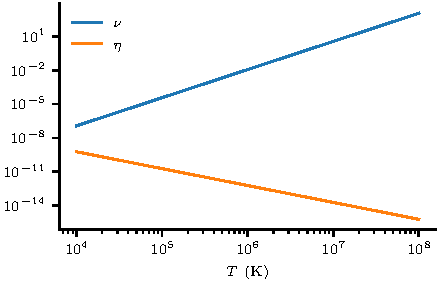
\includegraphics[width=\linewidth]{visc_dep_on_temp.pdf}
      \caption{Dependence of $\eta_0$ and corresponding Reynolds number $Re$ on temperature. Typical values used in the calculation of $Re$ are a field strength of $B = 5$mT, a length of $L = 1$Mm and a density of $\rho = 1.67 \times 10^{-12}$.}
      \label{fig:visc_dep_on_temp}
    \end{subfigure}
\caption{Dependence of transport parameters on magnetic field strength and temperature.}
\label{fig:visc_dep}%
\end{figure}

The parallel viscosity coefficient $\eta_0$ is identical to the dynamic viscosity coefficient of an unmagnetised plasma and depends on the ion number density $n$, temperature $T$ and collision time $\tau$ via the expression,
\begin{equation}
  \label{eq:parallel_visc_coeff}
  \eta_0 = 0.83 \times 10^{-10} n T \tau \text{kg m}^{-1}\text{s}^{-1},
\end{equation}
or,
\begin{equation}
  \label{eq:parallel_visc_coeff2}
  \eta_0 = 0.68 \times 10^{-16} T^{5/2} \text{kg m}^{-1}\text{s}^{-1}.
\end{equation}
Figure~\ref{fig:visc_dep_on_temp} shows the dependence of $\eta_0$ on temperature over a range of typical coronal temperatures, along with the dependence of a typical Reynolds number on temperature. Even at moderate temperatures of $10^6$, the coefficient of viscosity remains sizeable. As shall be explored later, this is in contrast to the value of resisitvity, which remains relatively small over this temperature range. This has implications for theoretical predictions of dominant dissipation mechanisms in the corona.

For simplicity, the dimensionless quantity $x = \omega \tau$ is used in the expressions for the remaining transport parameters, as is done in~\cite{braginskiiTransportProcessesPlasma1965} and all coefficients have identical units to $\eta_0$. The two perpendicular coefficients are written,
\begin{equation}
  \label{eq:perp_visc_coeff}
  \eta_2(x) = \frac{\eta_0}{0.96 \Delta} \left( \tfrac{6}{5} x^2 + 2.23 \right), \quad \eta_1 = \eta_2(2x),
\end{equation}
where
\begin{equation}
  \label{eq:delta}
\Delta = 2.23 + 4.03x^2 + x^4.
\end{equation}
The drift coefficients are written,
\begin{equation}
  \label{eq:drift_visc_coeff}
  \eta_4(x) = \frac{\eta_0}{0.96 \Delta} x \left( x^2 + 2.38 \right), \quad \eta_3 = \eta_4(2x).
\end{equation}
The relative strength of the five terms is important in considering which are most significant in the solar corona. The drift coefficients are of the order $\eta_0/(\omega \tau)$ and the perpendicular coefficients are of the order $\eta_0/(\omega \tau)^2$.

The origin of each of the five viscosity components can be understood by considering the effect of velocity gradients and collisions on a plasma from a kinetic perspective. As illustrated by Hollweg~\cite{hollwegViscosityMagnetizedPlasma1985}, the parallel viscous stress can be modelled as the result of pressure anisotropies being repartitioned by particle collisions. The drift terms are products of the velocity gradient perturbing particle orbits which generates pressure anisotropies and, in the absence of collisions, produces a stress which is orthogonal to the strain, resulting in no viscous dissipation. The inclusion of collisions again acts to repartition the anisotropies in the pressure giving rise to the perpendicular terms. This is explored in detail by Kaufman in~\cite{kaufmanPlasmaViscosityMagnetic1960}.

While it is illustrative to understand in a kinetic way why the drift terms produce no dissipation, it can be shown explicitly for the terms given in equation~\ref{eq:drift_terms}. The strain rate tensor can be written as the sum of only the parallel and perpendicular terms, $\ten{W} = \ten{W}^{(0)} + \ten{W}^{(1)} + \ten{W}^{(2)}$. As a result, both the drift stresses are orthogonal to $\ten{W}$ and by equation~\ref{eq:viscous_heat_generation2}, they produce no viscous dissipation. Furthermore, the relative size of the transport coefficients ($\eta_3 \propto \eta_0/(\omega\tau)$) suggests the drift terms may be completely neglected. While the drift terms can still meaningfully participate in certain dynamics~\cite{dellarPlanarChannelFlow2011,ferraroFiniteElementImplementation2006}, this thesis is broadly focused on the impacts of viscosity on coronal heating and so the drift terms will be neglected throughout the remainder of this work. While a similar argument suggests the perpendicular terms should also be neglected ($\eta_1 \propto \eta_0/(\omega\tau)^2$), these terms are required to rewrite the Braginskii tensor in a form useful for numerical simulation, as discussed later.

\subsection{Limit of strong magnetic field}

As already discussed, in an solar active region, $\omega \tau \approx 10^5 \gg 1$ and the transport coefficients in equations~\ref{eq:perp_visc_coeff} and~\ref{eq:drift_visc_coeff} become negligibly small compared to the parallel coefficient. As a result, the strong-field approximation to the Braginskii tensor is written,
\begin{equation}
  \label{eq:strong_field_approx}
\ten{\sigma}_{\text{brag}} = \eta_0 \ten{W}^{(0)} = \tfrac{3}{2} \eta_0 (\ten{W} \vec{b} \cdot \vec{b} ( \vec{b} \otimes \vec{b} - \tfrac{1}{3} \ten{I}).
\end{equation}
In a local coordinate system where the magnetic field is aligned with $b$, the tensor is
\begin{equation}
  \label{eq:z_aligned_strong_field_approx}
\ten{\sigma}_{\text{brag}} = \tfrac{3}{2} \eta_0 \ten{W}_{zz} ( \text{diag}(0,0,1) - \tfrac{1}{3} \ten{I}),
\end{equation}
where diag$(a,b,c)$ is the diagonal $3\times3$ matrix with the values $a$, $b$ and $c$ along the diagonal. Notice that the only velocity gradient to enter into the above tensor is that which is aligned with the magnetic field (including gradients stemming from the compressional $\nabla \cdot \vec{u}$ term in the rate of strain tensor, equation~\ref{eq:rate_of_strain}). It can also be seen that the magnetic field has no effect on the component of viscosity parallel to the field; it is identical to the corresponding component in the isotropic stress tensor,
\begin{equation}
  \label{eq:z_aligned_iso}
  (\ten{\sigma}_{\text{iso}})_{zz} = (\ten{\sigma}_{\text{brag}})_{zz} = \eta_0 \ten{W}_{zz}.
\end{equation}
In the strong-field regime, the only motion damped by viscosity is non-uniform compression or dilation of the plasma. 

This approximation is valid even for more moderate, quiet sun condition, where values of the magnetic field, $B\approx 10^6$, and temperature, $T\approx 10^6$, give $\omega\tau \approx 10^4$~\cite{morganGlobalConditionsSolar2017}. Where this approximation fails is around magnetic null points, regions of the corona where the magnetic field vanishes. Null points are an abundant feature in the coronal magnetic field~\cite{edwardsNullPointDistribution2015} and participate in a number of important solar phenomena~\cite{massonNATUREFLARERIBBONS2009,moreno-insertisPLASMAJETSERUPTIONS2013,barnesRelationshipCoronalMagnetic2007}. Any general model of solar viscosity must go beyond the strong-field approximation and additionally incorporate viscosity in the limit of weak magnetic field.

\subsection{Limit of weak magnetic field}

While the full Braginskii tensor~\ref{eq:braginskii_tensor} suitably presents the natural separation of viscous responses into parallel, perpendicular and drift components, this form is unsuitable for numerical simulation when null points are present in the magnetic field. As the field strength goes to zero approaching a null point, the unit vector $b$ in equations~\ref{eq:braginskii_parallel_term}--\ref{eq:drift_terms} becomes mathematically undefined. Numerically, the calculation of $b$ near the null would involve division by the magnitude of the field, a quantity close to or exactly zero, leading to errors or complete failure of the numerical scheme. Even if a numerical implementation were to check for a locally small field, it's unclear how the viscous terms and transport coefficients, as written in the form of equation~\ref{eq:braginskii_tensor}, interact as the field strength tends to zero. By rewriting the tensor as
\begin{eqnarray}\label{eq:brag_new}
\ten{\sigma}_{\rm brag} = &&\frac{3\eta_0+\eta_1-4\eta_2}{2|\vec{B}|^4}(\ten{W}\vec{B}\cdot\vec{B})(\vec{B}\otimes\vec{B})\\% \label{new1} \\
\nonumber
& &+~ \frac{\eta_1-\eta_0}{2|\vec{B}|^2}(\ten{W}\vec{B}\cdot\vec{B})\ten{I}\\% \label{new2}\\
\nonumber
& &+~ \frac{\eta_2-\eta_1}{|\vec{B}|^2}[\ten{W}(\vec{B}\otimes\vec{B})+(\vec{B}\otimes\vec{B})\ten{W}] \\%\label{new3}\\
%& & +~\frac12\eta_3(\ten{ZW}-\ten{WZ}) \\
%& &+~\left(\eta_4-\frac12\eta_3\right)[(\ten{ZW}\vec{b})\otimes\vec{b} + \vec{b}\otimes(\ten{ZW}\vec{b})]  \\
\nonumber
& &+~ \eta_1\ten{W},%\label{new4}
\end{eqnarray}
the anisotropic terms and isotropic term are clearly separated. The grouping of terms and the explicit use of $\vec{B}$ rather than $\vec{b}$ allows a numerical implementation to explicitly check the local value of $|\vec{B}|$ and, if it's smaller than some threshold, manually set the anisotropic coefficients in equation~\ref{eq:brag_new} to zero, avoiding a division by $|\vec{B}|$.

\subsection{The transition from isotropic to anisotropic}

\begin{figure}[t]
  \centering
  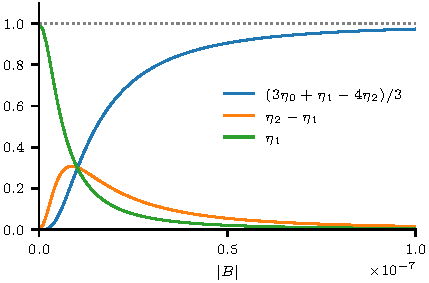
\includegraphics[width=0.5\linewidth]{brag_coeffs_2.pdf}
  \caption{Coefficients of the terms in equation~\ref{eq:brag_new2}, normalised against $\eta_0$.}%
  \label{fig:brag_coeffs2}
\end{figure}

The form of the Braginskii tensor as written in equation~\ref{eq:brag_new} is nearly in a form useful in understanding how quickly the tensor transitions from isotropic to anisotropic with changing magnetic field strength, since the isotropic component is completely isolated. Similarly, the parallel component can be isolated by further rewriting the tensor as,
\begin{eqnarray}\label{eq:brag_new2}
\ten{\sigma}_{\rm brag} = &&\frac{3\eta_0+\eta_1-4\eta_2}{3}\ten{W}^{(0)}\\% \label{new1} \\
\nonumber
& &+~ (\eta_2-\eta_1)[\ten{W}(\vec{b}\otimes\vec{b})+(\vec{b}\otimes\vec{b})\ten{W} - \frac{2}{3}(\ten{W}\vec{b}\cdot\vec{b})\ten{I}] \\%\label{new3}\\
\nonumber
& &+~ \eta_1\ten{W},%\label{new4}
\end{eqnarray}
Figure~\ref{fig:brag_coeffs2} presents the magnitudes of the coefficients of each of the terms in equation~\ref{eq:brag_new2}. Over the extremely small range between $|\vec{B}| = 0$ T and $10^{-7}$ T, the Braginskii tensor goes from completely isotropic to nearly completely parallel. Over the same range the coefficient corresponding to the perpendicular viscosity becomes relatively notable before tending to zero for large $|\vec{B}|$. The small transition region presents a problem in the numerical simulation of anisotropic viscosity, where the magnetic field strength likely changes more rapidly in space than can be captured by the coefficients in equation~\ref{eq:brag_new2}. 

In the simulations of magnetic null points found in chapter~\ref{chp:null_point_khi}, the magnetic field strength changes linearly in the $x$-direction. Given a typical grid spacing of $\Delta x = 0.01$, the jump in magnetic field from one grid point to the next is $5\times 10^{-5}$ T. This is much greater than the range over which the Braginskii tensor transitions between isotropic and anisotropic regimes and the viscous response is under-resolved as a result. For these simulations, the resolution would have to increase by a factor of $100$ to even begin to resolve the region of transition. Whether this region is physically significant is unknown, however, given the abundance of observable null points and their involvement in high-energy phenomena, it is possible that the isotropic (and perpendicular) viscosity near a null plays an important part in its dynamics. Computational solutions such as refining the mesh near the null or implementing a multigrid method may help to improve the resolution and better resolve the viscosity transition region, however these can be complex to implement in already existing codes. A simpler way to improve the resolution is to artificially scale $|\vec{B}|$ in the expression~\ref{eq:perp_visc_coeff} to enlarge the isotropic region to resolvable scales. While this approach is less physically realistic, its use may give a useful indication of how physically important the viscosity transition region is.

\section{Magnitude of transport parameters}

\subsection{Viscosity}

Hollweg~\cite{hollwegViscosityMagnetizedPlasma1985} gives $\eta_0 = 10^{-17} T^{5/2}\ \text{kg m}^{-1} \text{s}^{-1}$ for a Coulomb logarithm of 22 and $T$ given in units of Kelvin. For temperatures of $T=10^4$K to $T=10^8$K, $\eta_0$ ranges between $\eta_0 = 10^{-7} \text{kg m}^{-1} \text{s}^{-1}$ and $\eta_0 = 10^3 \text{kg m}^{-1} \text{s}^{-1}$. For the normalisation used in, for example, the kink instability chapter~\ref{chp:kink_instability} ($B_0 = 0.005\ \text{T}$, $L_0 = 10^6\ \text{m}$ and $\rho_0 = 1.67 \times 10^{-12}$) the Alfv\'en velocity is approximately $3.45 \times 10^6 \text{ms}^{-1}$ and, as a result, the range of the Reynolds number is $\text{Re} = \frac{V_A L_0 \rho_0}{\eta_0} = 5.67 \times 10^{-3}$--$5.67 \times 10^{7}$. For a more typical active region temperature of $T=10^6 \text{K}$, Re$=5.67 \times 10^2$. 

TODO graph of Reynolds number against temperature.

\subsection{Resistivity}

Hollweg's expression for the resistivity is $D = 2 \times 10^{9} T^{-3/2} \text{m}^2 \text{s}^{-1}$. This assumes the electron temperature is the same as the ion temperature. A temperature of $T=10^6\ \text{K}$ results in $D = 2 \text{m}^2 \text{s}^{-1}$. This corresponds to a Lundquist number of $S = \frac{V_A L_0}{D} = 1.73 \times 10^{12}$. Including the effects of electron pitch-angle scattering or current-driven instabilities can increase the effective resistivity. Exactly how much the resistivity is generally increased by is debated and ultimately depends on the local plasma conditions. Estimates range over Lundquist numbers of $10^{4}$--$10^{8}$ [TODO Add reference to these estimates from Ian Craig's paper].

TODO figure out when to changes D to eta and eta0 to nu

It should be noted is the magnetic Prandtl number, the ratio of Lundquist to Reynolds number, could be as large as $\text{Pr}_m = 10^2$ at a temperature of $T=10^6\ \text{K}$, taking into account an extremely large increase in effective resistivity. Assuming a more moderate increase in effective resistivity, the magnetic Prandtl number could be as high as $10^{6}$. This suggests that viscous heating may be much more important in the corona than Ohmic heating.
